\documentclass{ldr-simple-gray}


%------------------------------------------------------------
%首页start
\title{毕业论文开题报告}

\subtitle{基于Deep Koopman算子网络的非线性系统强化学习研究}
% \subtitle{基于Koopman理论的非线性系统强化学习研究}

\author{许忞欢}

\institute[]
{
导师:赵东东\\
兰州大学\quad 信息科学与工程学院
}

\date{\today}

% \logo{
\includegraphics[height=1cm]{lzu_logo.png}}
\titlegraphic{
\includegraphics[height=1.5cm]{lzu_logo.png}}

%首页end
%------------------------------------------------------------



\begin{document}

%封面
\frame{\titlepage}

% 要把今天讲的研究背景、主要结果、价值和意义(贡献点)讲清楚

\section{研究背景}

\begin{frame}{非线性系统控制}
  \begin{center}
    \zihao{3} {主要难点所在}
  \end{center}
  \begin{enumerate}
    \item 系统建模、系统动态
    \item 全局线性化
    \item 控制器设计、调参
    \item 适应系统变化
  \end{enumerate}	
\end{frame}
\note{一般来说,对于线性系统的控制,是比较好实现的,可以应用的方法也很多。但是在非线性系统中,控制就会变得困难。首先,与线性系统不一样的是,它的系统动态难以预测,不利于控制。广泛采用的研究方法是:在研究系统局部动态时,采用局部线性化的方式,使用线性系统控制手段在小范围内研究,而不是采用全局线性化;此外,控制器的设计,参数的调整都需要耗费时间和精力。最后,对于可能会因为自身的随机性而产生变化的系统而言,如何使得设计好的控制器,有能力适应新的环境也同样构成问题。应对上述困难,我设想在使用强化学习训练控制器的同时,引入koopman算子理论和深度Koopman网络缓解强非线性带来的影响。}

\begin{frame}{强化学习控制理论}
  \begin{figure}
    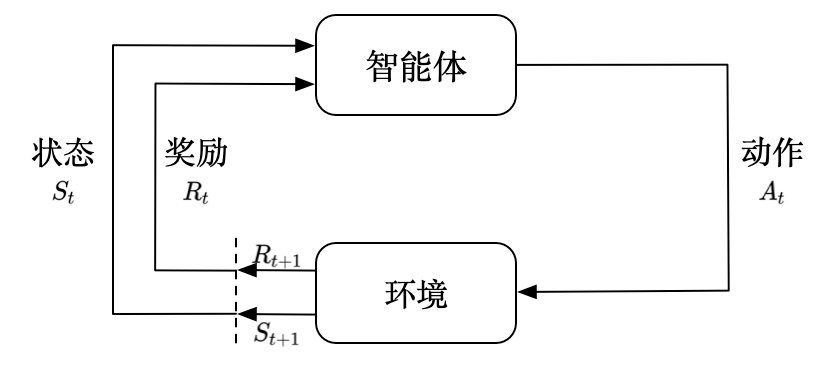
\includegraphics[width=0.5\textwidth]{RL-intro.png}
    \caption{强化学习基础框架}
  \end{figure}
  \begin{columns}
    \column{0.49\textwidth}
      \Large
      优点
      \normalsize
      \begin{enumerate}
	\item 无模型学习
	\item 对环境变化的适应性
	\item 处理连续的状态和动作空间
      \end{enumerate}

    \column{.02\textwidth}
    \rule{.3mm}{0.33\textheight}

    \column{0.49\textwidth}
      \Large
      缺点
      \normalsize
      \vspace{8pt}
      \begin{enumerate}
	\item 非线性系统动态难以控制
	\item 缺乏可控时的可解释性
      \end{enumerate}
      \vspace{8pt}
  \end{columns}

\end{frame}
\note{强化学习的工作中,训练完善的智能体应当在观测到环境的状态信息时,迅速给出合理的动作,并交由受控体执行,以达到控制的目的;同时,其训练过程可以被描述为:通过接收环境给出的状态计算对应的奖励,在规定的算法下,更新智能体的策略,以达到最大奖励的目标。实施强化学习控制的优点在于以下三点:1. 支持无模型学习,可以在系统模型未知的情况下进行策略的学习;2. 对环境的适应性好,只要规划好一个合适的奖励函数,就能让智能体在复数个环境中学习对应的最优控制策略;3. 支持连续和离散系统控制,连续时使用确定性策略,而离散时使用随机性策略进行训练和控制。}

\begin{frame}{Koopman算子理论全局线性化}
    \begin{figure}
	  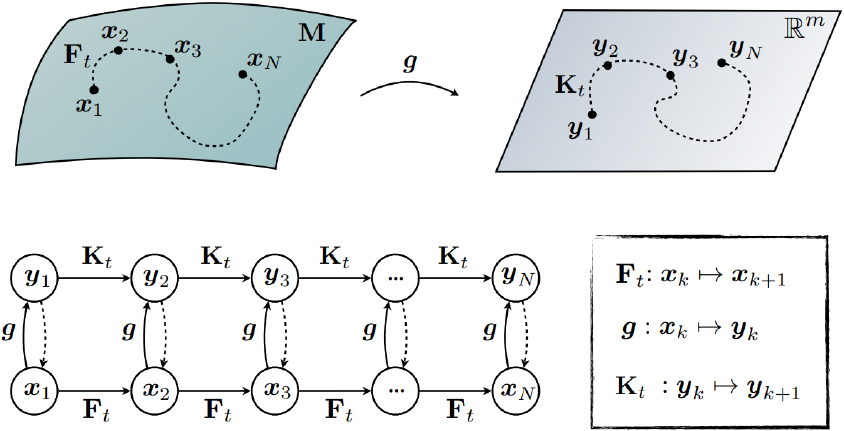
\includegraphics[width=0.65\textwidth]{koopman-theory.png}
	  \caption{非线性系统中Koopman算子的应用}
    \end{figure}
    \begin{itemize}
      \item $g$:\quad Koopman观测函数:一组基底,如($x_1, x_2, x_1^2,x_2^2,x_1x_2,\dots$)
      \item $K_t$:\quad Koopman算子:推进系统动态
    \end{itemize}
\end{frame}
\note{Koopman算子理论是一种可以实现非线性系统全局线性化,并通过线性变换预测系统动态的数学理论。在控制理论中的应用主体由嵌入函数和Koopman算子组成:其中,观测函数指的是一组非线性的变换基底,一般维度都比原非线性系统高,它将非线性系统嵌入到线性系统中,线性系统的基底就由观测函数组成。而koopman算子负责推进系统演化,在这里,koopman算子是数据驱动的,也就是通过接触到真实系统数据,拟合koopman算子,直至能够准确预测系统动态的。}


\section{研究内容}

% \begin{frame}{创新点}
%   \large
%   Koopman算子与强化学习
%   \normalsize
%   \begin{itemize}
%     \item 使得强化学习模型更好地把握非线性系统动态
%     \item 保留了非线性控制方法的“可解释性”
%   \end{itemize}
%   \large
%   深度Koopman网络
%   \normalsize
%   \begin{itemize}
%     \item 建立一个深度学习框架同时学习观测函数和Koopman算子
%     \item 添加一个辅助网络实现对于非线性控制变量的编码
%     
%   \end{itemize}
% \end{frame}

\begin{frame}{强化学习中的Koopman算子}
  \begin{figure}
    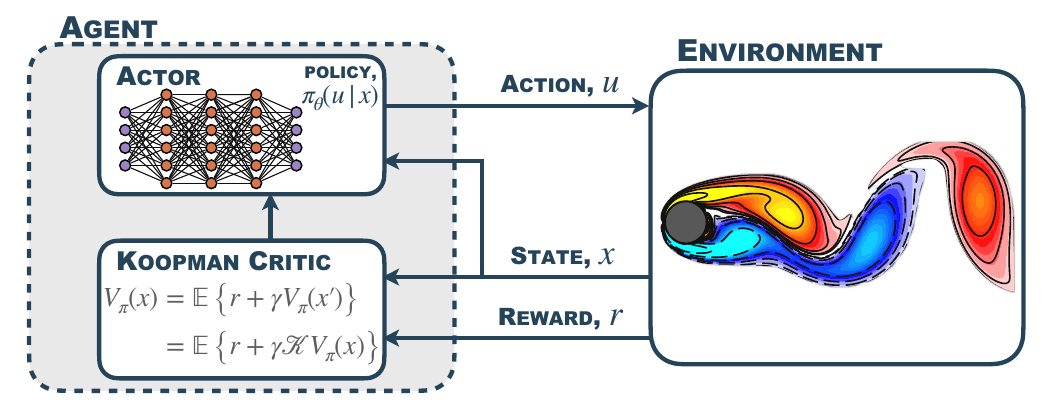
\includegraphics[width=0.9\textwidth]{sakc.png}
    \caption{强化学习中的Koopman算子\footfullcite{rozwood2023koopman}}
  \end{figure}
  Koopman-Critic接收状态和奖励,将这些信息提升到高维线性空间,
  以Koopman算子线性推进系统动态。
\end{frame}

\begin{frame}{深度Koopman算子}
  \begin{columns}
    \column{0.6\textwidth}
    \begin{figure}
      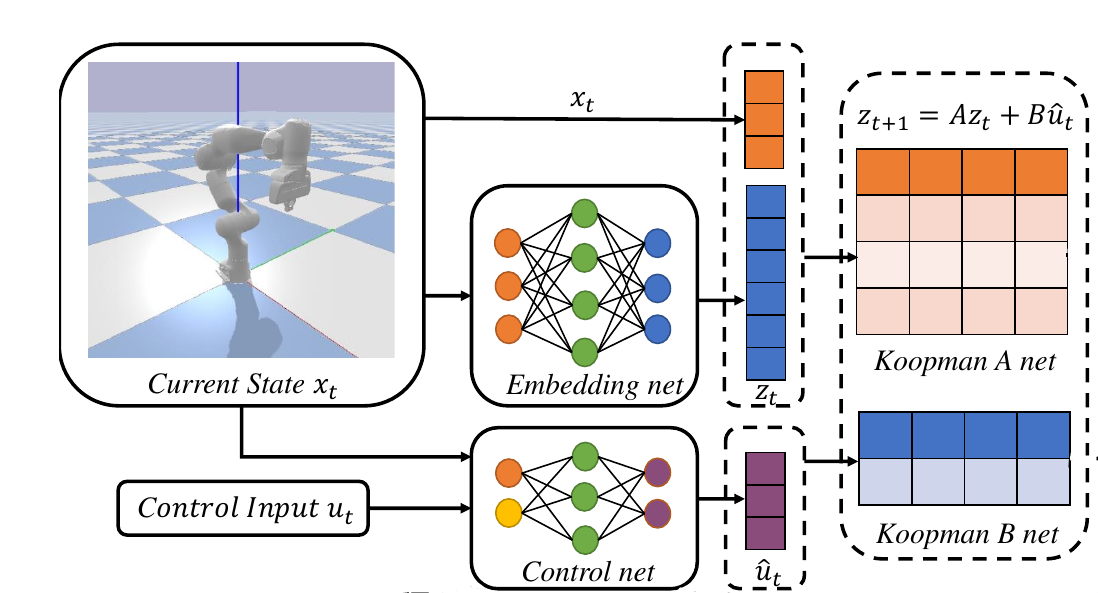
\includegraphics[width=\textwidth]{dkn.png}
      \caption{深度Koopman算子\footfullcite{shi2022deep}}
    \end{figure}
    \column{0.4\textwidth}
    以神经网络接管观测函数和Koopman算子
    (图中分别对应Embedding Net 和 Koopman A/B Net)
  \end{columns}
\end{frame}


\begin{frame}{价值和意义}
    \begin{itemize}
        \item 一种新的控制方法
        \item 面对强非线性具备可解释性
        \item 调试方便、部署难度低
    \end{itemize}
\end{frame}
\note{
  我的研究内容主要由两部分组成:
  第一,使用koopman算子,使得使得强化学习模型更好地把握非线性系统动态,同时保留了非线性系统控制方法的“可解释性”。
  如图所示的是加入了koopman算子的强化学习算法Actor-Critic的图解示意图,
  其中,Koopman-Critic部分接收状态和奖励,将这些信息提升到高维线性空间,以Koopman算子线性推进系统动态,
  使得强化学习训练过程中对于非线性系统下一时刻系统状态的价值期望值,也就是图中的$V_{pi}(x^')$的估计能够更加准确。
  第二,建立一个深度学习框架同时学习观测函数和Koopman算子,并添加一个辅助网络实现对于非线性控制变量的编码,
  而不是使用单位反馈的方式输入到koopman算子中,使得系统的状态非线性和动作非线性都得到了考虑,从而增加了系统信息的完整性。
}

\section{研究计划}

\begin{frame}{现有进度与规划}
  \begin{center}
    \Large
    目前进度
    \normalsize
  \end{center}
  \begin{itemize}
    \item 数据驱动的Koopman算子,如DMD,EDMD等算法;
    \item Soft Actor-Critic 算法及其代码实现。
  \end{itemize}  

  \begin{center}
    \Large
    未来工作
    \normalsize
  \end{center}
  \begin{itemize}
    \item 挑选合适的gym环境训练出Deep Koopman Network;
    \item 将DKN嵌入 Actor-Critic 类算法,训练合适的策略;
    \item 实验验证,并改进控制器构架;
    \item 借助ROS,尝试在机械臂上使用本算法进行控制。
  \end{itemize}  
\end{frame}
\note{}

\begin{frame}{\quad}
\begin{center}
   \zihao{2} 谢\quad 谢!
\end{center}

\end{frame}
\note{谢谢各位老师指点!!}

\end{document}
